\documentclass[11pt,a4paper,ngerman]{article}
\usepackage[bottom=2.5cm,top=2.5cm]{geometry} 
\usepackage{babel}
\usepackage[utf8]{inputenc} 
\usepackage[T1]{fontenc} 
\usepackage{ae} 
\usepackage{amssymb} 
\usepackage{amsmath} 
\usepackage{graphicx}
\usepackage{fancyhdr}
\usepackage{fancyref}
\usepackage{listings}
\usepackage{xcolor}
\usepackage{paralist}
\usepackage{fancyhdr}
\usepackage{subfigure}
\pagestyle{fancy}
\fancyhead[C]{Mikroprozessorpraktikum}
\fancyhead[L]{Protokoll 1}
\fancyhead[R]{WS 2011/12}
\fancyfoot{}
\fancyfoot[L]{}
\fancyfoot[C]{\thepage / \pageref{LastPage}}
\renewcommand{\footrulewidth}{0.5pt}
\renewcommand{\headrulewidth}{0.5pt}
\setlength{\parindent}{0pt} 
\setlength{\headheight}{15pt}


\author{Teilnehmer:\\ \\Marco Träger, Matr. 4130515\\Alexander Steen, Matr. 4357549}
\date{Gruppe: Freitag, Arbeitsplatz: HWP 1}
\title{Mikroprozessorpraktikum WS 2011/12\\ Aufgabenkomplex: 1}

\begin{document}

\lstset{language=c, basicstyle=\ttfamily\fontsize{9pt}{9pt}\selectfont\upshape, commentstyle=\rmfamily\slshape, keywordstyle=\rmfamily\bfseries, breaklines=true, frame=single, xleftmargin=3mm, xrightmargin=3mm, tabsize=2}

\maketitle
\thispagestyle{fancy}
\newpage
\section*{A 1.1 Output}

\begin{description}
	\item[A 1.1.1] Erläutern Sie unter Nutzung des User's Guide die Funktionalität der vier Register \\ \\
Alle der folgenden Register haben einen Ein-Byte-Wert, besitzen also jeweils eigene Werte für jeden Pin $x$ des Ports ($x = 0\ldots 7$).
		\begin{description}
			\item[P4SEL.x] selektiert für Bit $x$ des Ports 4 ob der I/O-Port oder die Funktion eines Peripheriegerätes genutzt werden soll
			\begin{description}
				\item[0:] I/O-Funktion
				\item[1:] Funktion je nach Peripheriegerät
			\end{description}
			\item[P4DIR.x] legt die Richtung des I/O Pins $x$ des Ports 4 fest
			\begin{description}
				\item[0:] Input (um ein Signal zu lesen)
				\item[1:] Output (um das Signal anzulegen)
			\end{description}
			\item[P4OUT.x] ist das Signal, das am Pin $x$ des Ports 4 anliegen wird, wenn man \texttt{P4DIR.x} = 1 und \texttt{P4SEL.x} = 0 setzt
			\item[P4IN.x] ist das Signal, das am Pin $x$ des Ports 4 anliegt, wenn \texttt{P4SEL.x} = 0. Ansonsten das Signal welches am \texttt{ModuleXOut} anliegt.
		\end{description}
	

	\item[A 1.1.2] Stellen Sie eine Liste der Operatoren zur Bitmanipulation auf. Erklären Sie die Möglichkeiten zum Setzen, Rücksetzen und Toggeln einzelner bzw. mehrerer Portleitungen eines Ports am Beispiel von P4OUT.  \\ \\
		\textbf{Operatoren:} \\ \\
		\begin{tabular}{l|l}
		Operation & Wirkung \\
		\hline \hline
		\texttt{x\&y} & Bitweises \texttt{UND} von \texttt{x} und \texttt{y} \\
		\texttt{x|y} & Bitweises \texttt{ODER} von \texttt{x} und \texttt{y} \\
		\texttt{x\textasciicircum y} & Bitweises \texttt{XOR} von \texttt{x} und \texttt{y} \\
		\texttt{\textasciitilde x} & Bitweises  \texttt{NOT} von \texttt{x} \\
		\texttt{x $<<$ y} & Linksshift von \texttt{x} um \texttt{y} Bits, es werden Nullen von Rechts eingefügt \\
		\texttt{x $>>$ y} & Rechtsshift von \texttt{x} um \texttt{y} Bits, es werden Nullen von Links eingefügt \\
		\end{tabular}
		\\ \\ \\
		Es gibt alle diese Operatoren auch mit einem folgenen Gleichzeichen, dabei wird das Ergebnis der Operation dem linken Operanden zugewiesen.\\ \\
		\textbf{(Rück-)Setzen von Bits:} \\ \\
		\begin{tabular}{l|l}
		Operation & Wirkung \\
		\hline \hline
		\texttt{P4OUT |= 1 $<<$ x}	 & setzt das x-te Bit von \texttt{P4OUT} \\
		\texttt{P4OUT \&= \textasciitilde(1 $<<$ x)} & setzt das x-te Bit von \texttt{P4OUT} zurück \\
		\texttt{P4OUT \textasciicircum= (1 $<<$ x)} & invertiert das x-te Bit von \texttt{P4OUT} \\
		\texttt{P4OUT |= maske} & setzt alle Bits von \texttt{P4OUT}, die in \texttt{maske} gesetzt sind\\
		\texttt{P4OUT \&= \textasciitilde maske} & setzt alle Bits von \texttt{P4OUT} zurück, die in \texttt{maske} gesetzt sind \\	
		\texttt{P4OUT \textasciicircum = maske} & invertiert alle Bits von \texttt{P4OUT}, die in \texttt{maske} gesetzt sind \\
		\end{tabular}
		
	\newpage
	\item[A 1.1.3] Erläutern Sie anhand der Abbildung der inneren Struktur einer Portleitung für die folgenden Registerbelegungen den Signalpfad und den Logikpegel der Portleitung P4.0. 
		\begin{lstlisting}[numbers=left]
# define LED_ROT (0x01)
// die Select-Einstellungen aller acht Portleitungen
// von P4 werden auf die I/O Funktion geschaltet
P4SEL = 0x00;
// die Richtung der unteren 4 Portleitungen 
// werden auf Out geschaltet
P4DIR = 0x0F;
// P4OUT.0 wird auf 1 gesetzt
P4OUT |= LED_ROT;
// also wird an Portleitung P4.0 eine 1 anliegen
		\end{lstlisting}
		
		Der Signalpfad ist dabei:
		\begin{figure}[h!]
			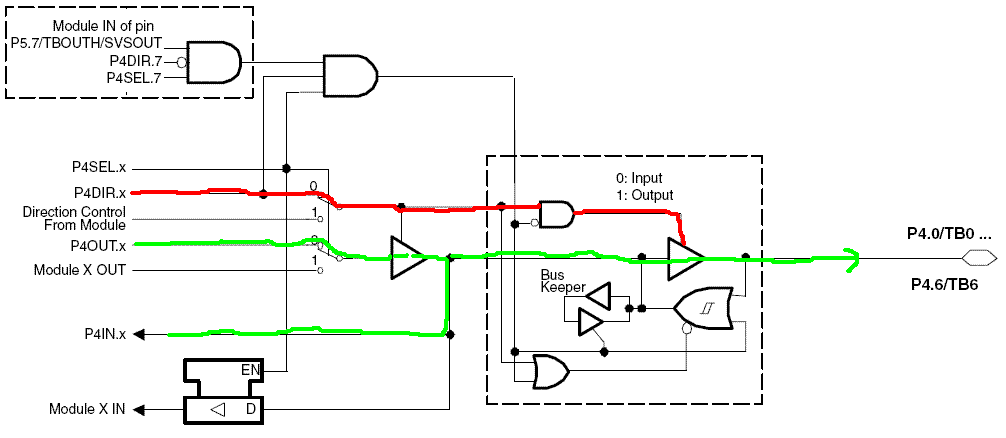
\includegraphics[scale=0.4]{0401011.png}
		\end{figure}	
	\item[A 1.1.4] Warum leuchtet eine LED am Port P4.0, wenn der Logikpegel "0" ist und nicht bei dem Logikpegel "1"? \\
	
		Betrachten wir die Abbildung des Schaltbildes für die LEDs: P4.0 ist dort mit P4B0 beschriftet, die LED am Port P4.0 mit LED1. An der LED1 liegt an der rechten Seite die Betriebsspannung an. Die linke Seite ist an die Betriebsspannung angeschossen	wenn der Logikpegel "1" ist. Wenn der Logikpegel "0" ist, ist die linke Seite an der Erdung angeschlossen. Wenn nun also der Logikpegel "0" anliegt, existiert eine Potentialdifferenz zwischen den beiden Seiten der Diode, also liegt über ihr eine Spannung an. Damit fließt Strom durch die LED und darum leuchtet sie. Wenn der Logikpegel "1" anliegt, liegt keine
	Potentialdifferenz vor.


	\item[A 1.1.5] Erläutern Sie inhaltlich die Bedeutung und Funktionalität der folgenden Codezeilen: \\
		\begin{lstlisting}[numbers=left]
unsigned char a;
#define LEDRT (0x01)
P4DIR = 0x00;
a = 10;
P4OUT = a;
P4OUT = 0x01;
P4DIR = 0x07;
P4OUT = 0x00;
P4OUT |= 0x01;
P4OUT |= LEDRT;
P4OUT ^= ~LEDRT;
P4OUT ^= LEDRT;
		\end{lstlisting}
		
		\begin{description}
		\item[Zeile 1] Deklaration einer nicht-vorzeichenbehafteten 8-Bit Variablen mit dem Namen a 
		\item[Zeile 2] Definition eines ALIAS für die 8-Bit Zahl 1, jedes Vorkommen des ALIAS wird  während der Übersetzung vom Precompiler durch die 8-Bit Zahl 1 ersetzt
		\item[Zeile 3] Stellt jede Portleitung des Port 4 auf Eingang (IN)
		\item[Zeile 5] Legt an Portleitung 1 und 3 von Port 4 eine 1 an, an alle anderen eine 0
		\item[Zeile 6] Legt an Portleitung 0 von Port 4 eine 1 an, an alle anderen eine 0
		\item[Zeile 7] Stellt Portleitung 0,1,2 von Port 4 auf Ausgang (OUT)
		\item[Zeile 8] Legt an Portleitung allen Portleitungen von Port 4 eine 0 an
		\item[Zeile 9] Legt an Portleitung 0 von Port 4 eine 1 an, an alle anderen eine 0
		\item[Zeile 10] Keine Veränderung (legt an Portleitung 0 von Port 4 eine 1 an, an alle anderen eine 0)
		\item[Zeile 11] Legt an allen Portleitungen von Port 4 eine 1 an
		\item[Zeile 12] Legt an Portleitung 0 von Port 4 eine 0 an, an allen anderen eine 1.
		\end{description}
		
		
	\item[A 1.1.6] Schreiben Sie ein kleines Programm, welches den Durchlauf einer Sequenz eines Ampelsignals mit den Phasen (Rot, Rot-Gelb, Grün, Gelb, Rot) simuliert. Nutzen Sie dazu die bereitgestellte Funktion wait() für eine Zeitschleife. Benutzen Sie eigene Macros und Operatoren zur Bitmanipulation.  \\ \\
	
		\begin{lstlisting}[numbers=left]
#define ROT 			~(0x01)
#define GELB  		~(0x02)
#define ROTGELB 	~(0x03)
#define GRUEN 		~(0x04)
#define WAITTIME	50000

void aufgabe116() {
	P4SEL = 0x00;
	P4DIR = 0x07;

	P4OUT = ROT;
	wait(WAITTIME);
	P4OUT = ROTGELB;
	wait(WAITTIME);
	P4OUT = GRUEN;
	wait(WAITTIME);
	P4OUT = GELB;
	wait(WAITTIME);
	P4OUT = ROT;
	wait(WAITTIME);
}
		\end{lstlisting}
		In den ersten Zeilen werden erst einige Konstanten definiert, sodass wir die Ampelfarben verständlicher im Code setzen können. In den Zeilen 9 und 10 werden die Leitungen von Port 4 auf die I/O-Funktion und auf Ausgang geschaltet, da hier die LEDs angeschlossen sind. Nun werden nach und nach die richtigen Farben für die Ampelphasen geschaltet (mit einer gewissen Verzögerung).
\end{description}

\newpage
\section*{A 1.2	Input}

\begin{description}
	\item[A 1.2.1] Erläutern Sie unter Nutzung des User's Guide die Funktionalität der sieben Register:
	
	\begin{description}
		\item[P1DIR] entscheidet, ob der jeweilige Pin als Eingang oder Ausgang fungiert, dabei beschreibt 0 einen Eingang, 1 einen Ausgang
		\item[P1IN] besteht aus einem Byte, deren Bits den aktuellen Logikpegel an dem jeweiligen Pin des Ports 1 darstellen
		\item[P1OUT] zeigt an dem jeweiligen Bit an, welcher Logikpegel an dem zugehörigen Port anliegen soll, falls P1DIR auf Ausgang und P1SEL auf I/O-Funktion geschaltet ist
		\item[P1SEL] gibt an, ob die einzelnen Pins des Port 1 direkt als I/O benutzt werden (Wert 0) oder für ein angeschlossenes Modul (Wert 1)
		\item[P1IE] de-/aktiviert die Intertupt-Flags (P1IFG) für die Pins des ersten Ports.
		\item[P1IES] entscheidet, ob man Interrupt durch eine low-high-Flanke (0) oder eine high-low-Flanke (1) auf dem jeweiligen Pin ausgelöst werden soll.
		\item[P1IFG] bezeichnet die Interrupt-Flags der Pins von Port 1. Ist ein Bit von P1IFG auf 1 gesetzt, so wurde von dem zugehörigen Pin ein Interrupt ausgelöst.
	\end{description}
	
	\item[A 1.2.2] Erläutern Sie die Funktion des Operators AND zur Bitmanipulation. Diskutieren Sie die Einsatzmöglichkeit am Beispiel einer IF-Anweisung \\
	
	Der AND-Operator (\&) führt Bit für Bit die Verundung der Bits der Arguments aus.\\
	\begin{lstlisting}
if (P1IN & Taster) {...}
	\end{lstlisting}
	Geht man für das Codebeispiel davon aus, dass an dem Pin $i$ von Port 1 ein Taster angeschlossen ist, so kann man durch Wahl der Variable \texttt{Taster} als Bitmaske, die nur an der Stelle $i$ eine 1 enthält (\texttt{Taster} = $2^i$), erreichen, dass die Abfrage genau dann erfolgreich ist, falls der Taster gedrückt wurde.
	
	\item[A 1.2.3] Erklären Sie die nachfolgenden Befehlszeilen und geben Sie an, welchen Wert die Variable a in den einzelnen Zeilen annimmt. \\
	
	\begin{lstlisting}[numbers=left]
#define Taster_rechts (0x01)
#define Taster_links (0x02)
P1DIR = 0x00;
P4DIR = 0xFF;
P4OUT = 0;
a = 7;
P4OUT = a;
P1OUT = a;
a = P1IN & 0x30; //beide Tasten gedr.
a = P1IN & 0x00; //Taste rechts gedr.
a = P1IN & 0x01; //Taste rechts gedr.
a = P1IN & 0x02; //Taste rechts gedr.
a = P1IN & 0x03; //Taste links gedr.
a = P1IN & 0x03; //beide Tasten gedr.
P4OUT = P1IN & Taster_rechts; //Taster an P1.0 nicht gedr.
P4OUT = P1IN & Taster_links; //Taster an P1.0 gedr.
	\end{lstlisting}
	\newpage
	\begin{description}
		\item[Zeile 1,2] Definiert Bitmasken, auf welche Bits der Register der rechte bzw. linke Taster zugreift
		\item[Zeile 3] Alle Pins von Ports 1 werden auf Eingang geschaltet
		\item[Zeile 4] Hier werden nun alle Pins von Ports 4 auf Ausgang geschaltet
		\item[Zeile 5] An alle Pins von Port 4 werden die Logikpegel 0 angelegt
		\item[Zeile 6] \texttt{a} wird auf 7 gesetzt
		\item[Zeile 7] Setzt die unteren drei Bits von \texttt{P4OUT} auf 1. Wenn \texttt{P4SEL} für die unteren drei Pins auf I/O-Funktion gestellt ist, liegt an diesen Pins nun jeweils eine 1 an (die LEDs leuchten nicht).
		\item[Zeile 8] Setzt die unteren drei Bits von \texttt{P1OUT} auf 1. Da \texttt{P1DIR} auf Eingang steht, ändert sich nichts.
		\item[Zeile 9] Da die beiden Tasten die beiden untersten Bits sind, ist das Ergebnis der Verundung 0, also wird a = 0 gesetzt
		\item[Zeile 10] Hier wird mit Und auf 0 ausgeführt, also wird a = 0 gesetzt
		\item[Zeile 11] a = 1, da Taster gedrückt
		\item[Zeile 12] a = 0, da mit der Bitmaske für den linken Taster verglichen wird
		\item[Zeile 13] a = 2, weil der Wert des linken Tasters genommen wird (an der zweiten Stelle in der Maske)
		\item[Zeile 14] a = 3, da sowohl der Wert des linken Tasters (2) und des rechten (1) genommen wird
		\item[Zeile 15] \texttt{P4OUT} wird auf 0 gesetzt, da kein Taster gedrückt ist
		\item[Zeile 16] \texttt{P4OUT} wird auf 0 gesetzt, da die Bitmaske den Tasterwert von P1.0 nicht berücksichtigt
	\end{description}
	
	\item[A 1.2.4] Schreiben Sie ein Programm, das die Ampelphasen simuliert. \\
	
	\begin{lstlisting}[numbers=left]
	#define Taster_rechts (0x01)
	#define Taster_links (0x02)
	#define rot (0x01)
	#define gelb (0x02)
	#define gruen (0x04)
	
void aufgabe_1_2_4() {
	// Letzten beiden Pins von Port 1 (Taster) als I/O-Input verwenden
	P1SEL &= ~0x03;
	P1DIR &= ~0x03;
	// Letzten drei Pins von Port 4 (LEDs) als I/O-Output verwenden
	P4SEL &= ~0x07;
	P4DIR |= 0x07;
	
	if (~((P1IN & Taster_rechts) ^ (P1IN & Taster_links))) {
		// Beide Tasten bzw. keine von beiden
		P4OUT &= ~gelb;
	} else if((P1IN & Taster_rechts) & ~(P1IN & Taster_lins)) {
		// Rechte Taste
		P4OUT &= ~gruen;
	} else if(~(P1IN & Taster_rechts) & (P1IN & Taster_lins)) {
		// Linke Taste
		P4OUT &= ~rot;
	}
}
\end{lstlisting}

\end{description}
\newpage
\section*{A 1.3 Ampel}
\begin{description}
\item[A 1.3.1] Nutzen Sie alle drei LED und den rechten Taster (P1.0), um eine Fußgängerampel zu programmieren. \\

\begin{lstlisting}[numbers=left]
	#define Taster_rechts (0x01)
	#define rot (0x01)
	#define gelb (0x02)
	#define gruen (0x04)
	
void aufgabe_1_3_1() {
	// Letzten beiden Pins von Port 1 (Taster) als I/O-Input verwenden
	P1SEL &= ~(Taster_rechts);
	P1DIR &= ~(Taster_rechts);
	// Letzten drei Pins von Port 4 (LEDs) als I/O-Output verwenden
	P4SEL &= ~(rot+gelb+gruen);
	P4DIR |= (rot+gelb+gruen);
	
	// alle LEDs ausschalten
	P4OUT |= (rot+gelb+gruen)
	
	if (P1IN & Taster_rechts) {
		// Gelbe LED an
		P4OUT &= ~(gelb);
		wait(3000);
		// Gelb aus, rote LED an
		P4OUT |= gelb;
		P4OUT &= ~rot;
		wait(3000);
		// Zusaetzlich gelbe LED an
		P4OUT &= ~gelb;
		wait(3000);
		// Rot und Gelb aus, gruen an
		P4OUT |= (rot+gelb);
		P4OUT &= ~gruen;
		wait(3000);
		// Gruen aus
		P4OUT |= gruen;
		wait(5000);
	}
}
\end{lstlisting}
In diesem Programm werden einfach nacheinander die richtige LEDs an- bzw. ausgeschaltet, sodass wir eine Ampelablauf simulieren. Die waits verzögern dabei die Auswertung so, dass wir wahrnehmen können, in welcher Reihenfolge die LEDs an- und ausgeschaltet werden.
\end{description}

\newpage
\section*{A 1.4 Taster}
\begin{description}
\item[A 1.4.1] Entwickeln Sie einen Binärzähler \\

\begin{lstlisting}[numbers=left]
	#define Taster_rechts (0x01)
	#define Taster_links (0x02)
	#define rot (0x01)
	#define gelb (0x02)
	#define gruen (0x04)
	
unsigned char counter = 0;
	
void aufgabe_1_4_1() {
	// Letzten beiden Pins von Port 2 (Taster) als I/O-Input verwenden
	P1SEL &= ~(Taster_rechts+Taster_links);
	P1DIR &= ~(Taster_rechts+Taster_links);
	// Letzten drei Pins von Port 4 (LEDs) als I/O-Output verwenden
	P4SEL &= ~(rot+gelb+gruen);
	P4DIR |= (rot+gelb+gruen);
	
	if (P1IN & Taster_rechts) {
		// Rechte  Taste gedrueckt
		if (counter < 7) {
			// Mehr als 7 geht nicht
			++counter;
		}
	} else if (P1IN & Taster_links) {
		// Rechte  Taste gedrueckt
		if (counter > 1) {
			// Weniger als 1 geht nicht
			--counter;
		}
	}
	// Korrekte LEDs setzen:
	// Wertigkeiten der LEDs sind gespiegelte
	// Wertigkeit der Bits von counter
	P4OUT &= ~(((counter & 0x01) << 2) + ((counter & 0x02) << 1) + (counter & 0x04))
	wait(100);
}
\end{lstlisting}
Das Prellen der Kontakte bewirkt, dass mehr Phasenübergange (Flanken) wahrgenommen werden, als tatsächlich vorkommen sollen. Dieses Problem kann man dadurch umgehen, dass man nach dem Verarbeiten eines Tastendrucks eine gewisse Zeit wartet um auf die Stabilisierung des Tasterpegels zu warten. Wir haben die Wartezeit experimentell ermittelt, sodass die Wartezeit die kleinste ist, bei der das Problem nicht mehr auftritt.
\end{description}
\label{LastPage}
\end{document}